\selectlanguage{english}%

\chapter{Introdução}

\indent Desenvolver controladores para sistemas não-lineares é quase sempre uma tarefa dispendiosa e complexa. Para plantas multivariáveis essa complexidade é ainda maior. É por esse motivo que é prática comum recorrer-se à linearização das equações que as descrevem, o que fornece uma aproximação do sistema inicial num formato que se encaixa às teorias de controle convencionais.

A linearização simples, realizada por meio da série de Taylor, resulta uma aproximação excelente localmente. No entanto, à medida que as variáveis controladas e manipuladas se afastam do ponto de operação, condição na qual foi realizada a linearização, o modelo passa a se afastar da planta real.

Neste cenário, a abordagem fuzzy figura como excelente ferramenta para solução destes desvios. Aparecendo pela primeira vez em \cite{zadeh65}, foi aplicada à modelagem de sistemas em \cite{takagi_sugeno}. Seus métodos consistem na linearização simples do sistema em mais de um ponto, baseados em um conjunto de métricas relevantes para o problema em questão. Desenvolve-se então um conjunto de regras para determinar o grau de pertinência do estado do sistema à cada um dos pontos pré-modelados. Utiliza-se então como modelo a soma ponderada das linearizações por estes coeficientes de pertinência. 

O objeto de estudo deste trabalho será o sistema de quatro tanques, desenvolvido por \cite{johansson2} com o objetivo didático de demonstrar de forma ilustrativa conceitos e propriedades de sistemas com múltiplas entradas e saídas (MIMO, do inglês \textit{multiple input, multiple output}). Seu diagrama esquemático é apresentado na  \hyperref[fig4tank]{Figura \ref{fig4tank}}. Ele consiste em quatro tanques interconectados, um reservatório inferior, quatro válvulas esferas e duas bombas de corrente contínua que bombeiam o fluido do reservatório inferior para os tanques de forma cruzada, de acordo com a razão entre os fluxos definida pela posição das válvulas.

O sistema de quatro tanques é não linear. Seu modelo linearizado apresenta um zero multivariável que pode estar localizado tanto no semi-plano esquerdo quanto no semi-plano direito dependendo da configuração das válvulas. A abertura das válvulas determina se o sistema é de fase mínima ou de fase não-mínima afetando a estratégia de controle a ser adotada.

O objetivo é controlar os níveis do fluido nos tanques inferiores 1 e 2. As entradas do processo são as tensões de entrada das bombas, e as saídas são os níveis de fluido nos tanques 1 e 2. As demais variáveis de processo são os níveis do fluido nos tanques 3 e 4, os fluxo da bomba e a razão entre os fluxos para os tanques. 

Este trabalho está organizado da seguinte forma: Na \hyperref[secModConvencional]{Seção \ref{secModConvencional}} é feita a modelagem matemática do sistema não linear e sua linearização em torno do ponto de operação em estado estacionário.A  \hyperref[secModFuzzy]{Seção \ref{secModFuzzy}} apresenta os conceitos da modelagem fuzzy e sua aplicação na planta. Na seção seguinte é feita uma análise comparativa entre os modelos desenvolvidos. Por fim, algumas considerações finais e sugestões de trabalhos futuros são apresentadas na \hyperref[secConclusao]{Seção \ref{secConclusao}}.

\begin{figure}
	\begin{centering}
		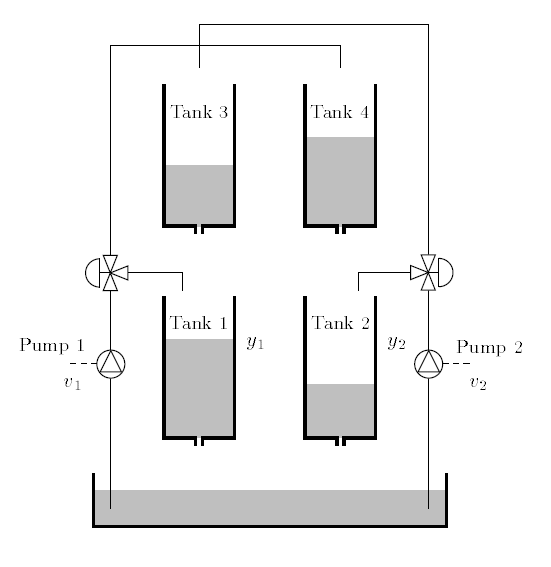
\includegraphics[width=0.5\textwidth]{figs/4tank.png}
		\par\end{centering}
	\caption{\label{fig:teste_fig_01}Diagrama esquemático do sistema de quatro tanques e planta didática}
\end{figure}

\indent Desenvolver controladores para sistemas não-lineares é quase sempre uma tarefa dispendiosa e complexa. Para plantas multivariáveis essa complexidade é ainda maior. É por esse motivo que é prática comum recorrer-se à linearização das equações que as descrevem, o que fornece uma aproximação do sistema inicial num formato que se encaixa às teorias de controle convencionais.

A linearização simples, realizada por meio da série de Taylor, resulta uma aproximação excelente localmente. No entanto, à medida que as variáveis controladas e manipuladas se afastam do ponto de operação, condição na qual foi realizada a linearização, o modelo passa a se afastar da planta real.

Neste cenário, a abordagem fuzzy figura como excelente ferramenta para solução destes desvios. Aparecendo pela primeira vez em \cite{zadeh65}, foi aplicada à modelagem de sistemas em \cite{takagi_sugeno}. Seus métodos consistem na linearização simples do sistema em mais de um ponto, baseados em um conjunto de métricas relevantes para o problema em questão. Desenvolve-se então um conjunto de regras para determinar o grau de pertinência do estado do sistema à cada um dos pontos pré-modelados. Utiliza-se então como modelo a soma ponderada das linearizações por estes coeficientes de pertinência. 

O objeto de estudo deste trabalho será o sistema de quatro tanques, desenvolvido por \cite{johansson2} com o objetivo didático de demonstrar de forma ilustrativa conceitos e propriedades de sistemas com múltiplas entradas e saídas (MIMO, do inglês \textit{multiple input, multiple output}). Seu diagrama esquemático é apresentado na  \hyperref[fig4tank]{Figura \ref{fig4tank}}. Ele consiste em quatro tanques interconectados, um reservatório inferior, quatro válvulas esferas e duas bombas de corrente contínua que bombeiam o fluido do reservatório inferior para os tanques de forma cruzada, de acordo com a razão entre os fluxos definida pela posição das válvulas.

O sistema de quatro tanques é não linear. Seu modelo linearizado apresenta um zero multivariável que pode estar localizado tanto no semi-plano esquerdo quanto no semi-plano direito dependendo da configuração das válvulas. A abertura das válvulas determina se o sistema é de fase mínima ou de fase não-mínima afetando a estratégia de controle a ser adotada.

O objetivo é controlar os níveis do fluido nos tanques inferiores 1 e 2. As entradas do processo são as tensões de entrada das bombas, e as saídas são os níveis de fluido nos tanques 1 e 2. As demais variáveis de processo são os níveis do fluido nos tanques 3 e 4, os fluxo da bomba e a razão entre os fluxos para os tanques. 

Este trabalho está organizado da seguinte forma: Na \hyperref[secModConvencional]{Seção \ref{secModConvencional}} é feita a modelagem matemática do sistema não linear e sua linearização em torno do ponto de operação em estado estacionário.A  \hyperref[secModFuzzy]{Seção \ref{secModFuzzy}} apresenta os conceitos da modelagem fuzzy e sua aplicação na planta. Na seção seguinte é feita uma análise comparativa entre os modelos desenvolvidos. Por fim, algumas considerações finais e sugestões de trabalhos futuros são apresentadas na \hyperref[secConclusao]{Seção \ref{secConclusao}}.

\selectlanguage{brazil}%

